\documentclass[12pt, a4paper]{memoir} % for a short document
\usepackage[english]{babel}
\usepackage [vscale=0.76,includehead]{geometry}              
\usepackage{fullpage}
\usepackage{mathptmx} % font = times
\usepackage{helvet} % font sf = helvetica
\usepackage[latin1]{inputenc}
\usepackage{relsize}
\oddsidemargin 0.0cm  
\evensidemargin 0.0cm  
\textwidth 17cm 
\topmargin -1cm 
\textheight 23.5cm
\usepackage{graphicx}
\usepackage{float} 
\usepackage{multimedia}
\usepackage{amsmath,amssymb}
\usepackage{listings}
\usepackage{graphicx} % Allows including images
\usepackage{booktabs} % Allows the use of \toprule, \midrule and \bottomrule in tables
%\usepackage[nottoc, notlof, notlot]{tocbibind}
\usepackage{amsfonts}
\usepackage{amsmath,bm}
\usepackage{hyperref}
\usepackage[round]{natbib}
\lstset{
  numbers=left,   
  firstnumber=1,
  numberfirstline=true,
  language=C, 
  frame=L
  } 



\bibliographystyle{plain}

%\headstyles{komalike}
\nouppercaseheads
\chapterstyle{dash}
\makeevenhead{headings}{\sffamily\thepage}{}{\sffamily\leftmark} 
\makeoddhead{headings}{\sffamily\rightmark}{}{\sffamily\thepage}
\makeoddfoot{plain}{}{}{} % Pages chapitre. 
\makeheadrule{headings}{\textwidth}{\normalrulethickness}
%\renewcommand{\leftmark}{\thechapter ---}
\renewcommand{\chaptername}{\relax}
\renewcommand{\chaptitlefont}{ \sffamily\bfseries \LARGE}
\renewcommand{\chapnumfont}{ \sffamily\bfseries \LARGE}
\setsecnumdepth{subsection}


% Title page formatting -- do not change!
\pretitle{\HUGE\sffamily \bfseries\begin{center}} 
\posttitle{\end{center}}
\preauthor{\LARGE  \sffamily \bfseries\begin{center}}
\postauthor{\par\end{center}}

\newcommand{\jury}[1]{% 
\gdef\juryB{#1}} 
\newcommand{\juryB}{} 
\newcommand{\session}[1]{% 
\gdef\sessionB{#1}} 
\newcommand{\sessionB}{} 
\newcommand{\option}[1]{% 
\gdef\optionB{#1}} 
\newcommand{\optionB}{} 

\renewcommand{\maketitlehookd}{% 
\vfill{}  \large\par\noindent  
\begin{center}\juryB \bigskip\sessionB\end{center}
\vspace{-1.5cm}}
\renewcommand{\maketitlehooka}{% 
\vspace{-1.5cm}\noindent
\includegraphics[height=14ex]{logoINP.png}\hfill\raisebox{2ex}{
\includegraphics[height=7ex]{logoUJF.jpg}}\\
\bigskip
\begin{center} \large
Master of Science in Informatics at Grenoble \\
Master Math\'ematiques Informatique - sp\'ecialit\'e Informatique \\ 
option \optionB  \end{center}\vfill}
% End of title page formatting

\option{$<$GVR$>$}
\title{ Inverse Procedural Generation of Geological Stories}%\\\vspace{-1ex}\rule{10ex}{0.5pt} \\sub-title} 
\author{Garcia Maxime}
\date{ $<$June 23rd 2016$>$} % Delete this line to display the current date
\jury{
Research project performed at $<$INRIA Monbonnot$>$ \\\medskip
Under the supervision of:\\
$<$Dr. R\'emi Ronfard ,INRIA$>$\\\medskip
Defended before a jury composed of:\\
$[$Prof/Dr/Mrs/Mr$]$ $<$first-name last-name$>$\\
$[$Prof/Dr/Mrs/Mr$]$ $<$first-name last-name$>$\\
$[$Prof/Dr/Mrs/Mr$]$ $<$first-name last-name$>$\\
$[$Prof/Dr/Mrs/Mr$]$ $<$first-name last-name$>$\\
}
\session{$[$June$]$\hfill 2016}

\begin{document}
\selectlanguage{english} % french si rapport en français
\frontmatter
\begin{titlingpage}
\maketitle
\end{titlingpage}

\section{Abstract}

In this project we tackle the problem of restoring the complete history of a 2D geological 
subsurface also calls a cross-section. It is represented by a 2D sketch and we will produce a backward animation on it, starting
at the section current state going in the past while detecting and un-doing geological events
that possibly occured throught its history. \\
Several scenarios will be taken into account while keeping only the most plausible ones. The animation is the result of running a simulation using mass spring systems mapped on the different part of the cross-section.

\section{Introduction}

Hand-drawn sketches are very used in geology for illustrating and validating hypotheses. It is the main way of keeping and showing geological data. Indeed, showing an image of what we have in mind is a really good way to convey our thoughts, especially here in geology where we can draw from multiple points of view. Futhermore geologists write lots anotations on their drawing to give more hints and be more specific in the information they want to show in their sketchs. 
For instance sketches can be used to reconstruct a 3D view of the subsurface by drawing a 2D top view of the current terrain (2) and using anotations or to represent 2D vertical cross-sections. \\\\

However anotations are limited in explaining what happened in the past, it is difficult to anotate the past of the geological representation on a single sketches. Therefore geologists must draw several sketches when they whant to show the history of a terrain. \\\\

This exaclty what they do when they want to do cross section restoration (ref). It consists in drawing several sketches of the same cross section at different time steps starting from the its current state.  A cross section is composed of several geological elements especially blocks, layers and faults. The layers they draw correspond to different sedimentary layers that have deposited  along history. The faults correspong to breaks in the section and create discontinuities in it. They can be of three types:
. However as we are in the 2D vertical case we are only interesed in the inverse and normal faults. Finally blocks correspond to parts of the section which are between two faults or one fault and on boundary of the sketch. 
Here is an exemple of a geological skecth (eg): 


The current state of the cross section is the result of several geological phenomena such as erosion, foldings, sedimentations, fault impacts, etc..., which occured in the past at different time. Consequently, restoring a cross section can differ depending on the geologist point of view.
However using the initial sketch  and geometrical tools (ref) geologists are able to draw the past state of the cross section before any erosion, fault and sediment events and this restoration is usually unique and doesn't differ much between geologist.An analysis of the different layers and faults usually lead to the same geometrical evolution reconstruction which has been provoqued by compression or extension of the rock masses before, after or during deposit and erosion of the sediments and basement rocks. \\\\

The main problem geologist are facing in this restoration is to find (deduce) what really happened to go from the current state to the past one. They have two things to identify. First they have to find all the events that occured from the past to the current state. Then they have to find in with order they occured because it is possible that even when changing the event order we obtain the same restoration at the end. Futhermore it is possible to find the same restoration having identifying different events in two different hypothesis. \\\\

Consequently geologists have to draw lots of sketches in order to expose their hypothesis. In addtition those drawings are rather limited: on top of representing only one 2D cross-section of the terrain being investigated, they can only represent hypotheses on the underground geometry at discrete time steps, rather than a complete continuous history. Futhermore insuring consistency between these sketches over time heavily depends on available data, maturity of the regional geological interpretation and the skills of the geologist, i.e. his knowledge on the way rocks and sediments fold, on the way faults propagates and produce sliding and displacements, and on the way sediments are deposited or eroded, etc...\\\\


Recently, it was proposed to organize geological sketches into story trees to present and compare different interpretations of the formation of a given terrain (6) but the task remains labor-intensive, requiring the geologist to draw every sketch in the story tree. Moreover, even while being skillful and experienced, it’s hardly impossible to a geologist to express a continuum of the deformation of a geological cross-section with available tools.
In this internship, we would like to follow up on this line of research by proposing methods for inferring a geological story tree directly from one geological sketch, and presenting the resulting tree of possible geological stories as an animation.\\\\

\section{State of the Art}\\

Several solutions of very different kind have been proposed to solve the problem of correctly exposing many restoration hypothesis without inconsistencies and without spending too much time creating them. We distinguish two types of solutions: the geometrical ones and the mecanical ones.\\\\

Geometrical solutions consist in assuring only geometrical consistancy when exposing the solution while mecanical ones consist in running a physical simulation over the past cross section and see if the animation created confirm the hypothesis.

\section{Geometrical solutions}

Like mentionned above Lidal (ref) proposed a solution using trees to organize their resoning. Starting from the initial drawing the geologist can draw several stories where each node of the tree conctains a new sketch. However it is possible to (supperpose) the previous drawing to the new one helping keeping geometrical consitancy and reducing conciderably the time spent for drawing. Futhermore as geologists use usually seismic recording to draw the starting drawing, having this recording in background really help them in being consitent. As a result with fewer sketches and less time spent drawing, geologists  (see eg) can express their ideas better than with traditionnal sketching. Futhermore this tool is really efficient when exploring diifferent hypothesis because at each node we can create another branch to explore a new possibility and thus they can either refined their animation or try different scenarios. \\\\

However this solution doesn't necessarely keep the topological consistancy of drawing unless the geologist spend more time being carefull of having precise topological consistant drawings. This topological aspect can be important when validating hypothesis especially when they restore very old cross sections and the topology of the terrain undewent drastic changes(exemples?).

Recently VAC and VGC proposed a solution to have space-time topological consistancy in 2D drawings. More precisely it propose a solution for inbetweening two drawings of the same model which underwent topological changes. The fondation of the technique is the data structure VGC which has been shown to model all possible incidence relations between vertices, edges and faces in 2D sketches. Then the VAC are used to describe all possible changes in the topology of a vector graphic complex over time.\\\\\

Other geometrical tools such as move (ref) are used  to produce the restoration. They use geometrical and geological properties of the drawing and apply kinematic algorithms to deform the different blocks and moduli. They take into account several geological phenomena such as compaction, erosion, sedimentation and folding in order the keep the geological consistancy while the user is restoring interactively the cross section. They also consider more specific effects such as thermal subsidence and isostasy to have finer results in the restoration. In addition this kind of tool can be used for foward modeling which can help geologists to validate their hypothesis in the case they want to check if the restoration they produced can give the same result as today terrain situation. Futhermore they can consider the 3D aspect of a subsurface using several cross sections and a 3D model of the considered area. It is important to note that this kind of tool doesn't produce realisitc results in terms of physical aspect but they have fast computation time and let the user interact to build the restoration.\\\\\

Here is an example of the chartreuse restoration using that king of geometrical tools. Here it was done manually by a geologist who  dealt with each block one by one and flattenrf each layer while conserving their respective area or length. After the flattening operation the user can manually stick the new block to its neighbours with the corresponding moduli facing each other.

\section{Physical solutions}

In order to solve the cross-section restoration problem an other kind of solution tools has been explored which is physically based tools. While geometrical tool don't assure the physical consistancy of the restoration which can question the restoration itself, physical based tools are by nature physically consistent.  We can identify two kind of physically based tools: those which help validating 	complex structural model of 3D subsurface like LithoTect(ref) and those which run a simulation over simpler but physically coherent enough using finite element method with the Coulomb theory like SLAMTec and OptumG2.
Software like LithoTect are very usefull because they allow geologist to build very consistent and complex model of a subsurface which implies that they can create very fine 2D cross section where they can run a physical simulation on.
Software like SLAMTec or OptumG2 run simulations over simpler models which are also physically consistent but the simulation will take less parameters and properties of the terrain, leading to faster computation time .Such tools can be used to validate a restoration. Indeed by running a simulation over the restoration geologist can see if what they produce seems coherent with the current state of the cross section even if those simulations can never produce the same result as this current state. This is one drawback of using those tool of foward simulation, even if we have a very fine representation of our model it can never achieve to retrieve a very similar correspondances and cannot validate by itself a restoration, geologists have to discuss the solution proposed. However some physically based tool try to  solve this problem by proposing a backward simulation. This simulation is not simulating the "real" inverse of what happened to the current cross section but they run a finite element simulation with opposite forces and condition to what the geologist think that happened. For instance if the current section has been subject to compression forces the tool will apply extension forces to the model, same thing with compaction and other phenomena. While this method is likelly to produce much better results in terms of similarity with the restoration and the current state of the section, it is more difficult to use because there exist many uncertainties on identifying the events that occured between the current cross section and the restoration as there are several possible scenarios.

Even though those physically based tool respect physic laws and produce very consistent results, they are not fully matching the cross section current state and thus cannot validate the hypothetical section history they have simulated. In addition this kind of tool doesn't explore several scenarios and are restrained to a single or very few cases. 
That's why one of the main purpose of this master thesis is to explore and propose several plausible scenarios.

\section{Our Solution}

We presented two kinds of tools used for solving the problem of producing the animation between the recovered restoration and the current cross section. Moreover we can note that regardless the type of tool some of them produce forward animation and others backward ones. 
Here we will opt for a backward simulation using a hybrid tool between geometrical physical.
Thus we will run an inverse modeling animation on the current 2D section and compare it visually to the provided restoration.\\\\

In this master thesis the main objective is to create a generic tool which builds different scenarios from a given drawing. The tool must give the user choice to make and allow him to come back on them. That's why similarly to Lidal (ref) we will use story trees to encode our scenarios.

In order to produce such at tool we had to answer the following questions:
- What will be our input data (which format)
- How to precilly encode our scenarios and deal with them
- Which method to use for animating
- How to validate the solution proposed

Because the topology of the section is changing over time we opted for using VAC and VGC structures which we allow us to keep a time-space topological consistency during the animation.


For the story telling 

For the animation

The general workflow is


 In order to explore a reasonable number of geological scenarios we will encode them into an interactive story tree.\\\\

We first provide one possible scenario to the user making the story tree taking the form of a line. Starting from that point the user can decide to create another branch from any node and explore a new scenario. Each node of the tree will corresponds to a discrete topological event such as faults which can be dealt using a similar approach to (3). This means that between two consecutive node levels we will simulate the consequence of this event. Thus the tree banches will correspond to the continuous animation of the soil change caused by the end node event of the branch.\\\\

However discrete geological events are not the only phenomena we have to consider in order to represent all the plausible scenarios. Indeed continuous events such as erosion and sedimentation have to be taken into account. Those events will be integrated into the tree as branches.
More phenomena may be added during the internship but we have to be careful to not produce too many scenarios that are not relevent, therefore the number of considered phenomena should be moderated. However the number of unrelevent scenarios can be reduced by taking into account more geological laws that will restrict node and branch creations.
Thus at each node and branch creation, the user can only choose events among a restricted range. This property is important because it is time saving for geologists who want to see only the most plausible scenarios. In addition methods proposed for controlling the number of branches in the story tree (7) will be adapted for this geological case.\\\\

Before generating the tree we will extract all the information we can from the 2D section, that is to say the number of layers, their age, the already determined eroded zones and so on.\\\\

As geological structures can have a rather complex topology, the 2D section will be presented as a vector graphics complex representation (4) drawn using vpaint software like in Figure 3. This data structure has been shown to model all possible incidence relations between vertices, edges and faces in 2D sketches. More structures derivating from vector graphics complex will be implemented in order to take into account the geological aspect of the sketch.\\\\

The inverse modeling animation will be done on top of the vector animation complex structure (5) which is used to describe all possible changes in the topology of a vector graphic complex over time. This method will require prior information about several geological parameters that will affect the animation such as materials’ density, friction coefficients and others like erosion and sedimentation speeds.\\\\\

\section{Continuous Simulation}

\section{General Overview}

Here we will present our first method to tackle the problem of proposing a panel of plausible animations giving geological restoration as final state from a 2D input slice. 
The main idea of our methods is to map a mass spring system on each block (section between two or several faults) of the slice and simulate a extension by freezing the physics of several blocks at each time step and let the others move as they should given geological events. The output of our method we will a series of inbetween VGC which will be played on VPaint.\\\\
The first step of our method is to draw the 2D slice using VPaint which allow the user to do it pretty quickly.
This drawing will highlight all the different blocks which are contained in the slice.
In addition the VPaint drawing will show all the different layers of each block and faults. Additionnal information such as erosion lines can be added. \\\\
After drawing our section in VPaint we will read the .vec file in our GeoPaint editor in order to add all the necessary information about our section such as the layers' materials containing crutial information (density, age, etc...) or even  additionnal information about faults and erosion lines. This information will allow us to run the animation over our section.
Indeed once the geo editing is finished we will gather all the information into one format (.geo) and will use it to describe our slice and animate it.\\\\
The first step for animating is mapping a mass-spring system into each block. Then we have to solve the restoration problem at a geological point of view, that is to say build the first story tree and find a method to propose which event can happen at each node.\\\\
As the first proposed story tree is computed fully automaticaly it may not show the most plausible result that's why we propose the user to choose events a list of plausible geological events at each node.
This way the user can construct all the plausible stories he wants.

\section{General structure}

One important matter in our model is to choose carefully the representation of our slices as it will affect how we will animate it.
We choose one possible representation of a geological slice but we are aware that some part of this structure can be modified through the project progression.\\\\
Similary to the drawing a slice is composed of blocks, faults and erosion lines. It also contains a list of all the materials composing the different layers.This list will be usefull when we want to see if one material disappeared from one block. Each blocks is composed of layers and interlayers lines. Knowing all the interlayers is important to link the layer mapping together (see Animation Model section).\\\\
Each block contains a list of the materials composing its layers. Like said abbove we will compair it to the slice material to take into account erosion effect which cause layers to disappear. \\\\
Each layer contains its interlayers,left and right sides and also its corners which are important for linking blocks together during the animation. The layer contains also its material which gives a lot information for the animation (density, friction, erosion speed, sedimentation speed). 
In fact this information will be taken into consideration inside the mass spring system attached to the layer.
Each fault contains each line composing it. Sub faults which we know that came after an other can be added.


\section{Animation Model}

Like mentionned above the animation will be done by mapping a mass-spring system on each block. In fact it is more accurate to say that mass-spring system are mapped on layers instead of blocks. We proceed this way to take into account each layer orientation in the mapping as it is mapped according to layer's borders gradients. Considering that each layer is a rectangle that underwent some deformations the mapping will be done following the steps:	\\\\		
\indent	- First we have to put the masses both at the layer border but also inside it.\\\\
\indent	- We put the masses on the borders in an uniform way.\\\\
\indent	- We put the masses inside the layer: to do so we have two solutions:\\\\
\indent \indent	- Compute hermite curve between each pair mass of the two interlayer and place particles uniformly on those curves.\\\\
\indent \indent	- Compute the intersections between the previous hermite curves and the  one coming from each pair mass of the two sides and place particles at those intersections.\\\\
	Even if the second solution might show better results that the first one we have chance that the curve comming from the sides might be not inside the layer due to big deformation making the layer non convex. \\With the first solution this problem is unlikely to occur because of the type of the deformations. In either case the hermite curves be created using a mass pair and the gradient of the broder at each extremity as tangents. This way the layer will tend to transform back to a rectangle shape.\\\\
\indent	- Link particles with springs. \\We divide springs into 5 categories like described in \citep{cloth}: Vertical, Horizontal, DownShear, UpShear and Flexion. Adding flexion spring show better results in terms of shape preservation and breaking prevention. The resulting network looks like:\\
	
	\begin{figure}[H]
	\centering
	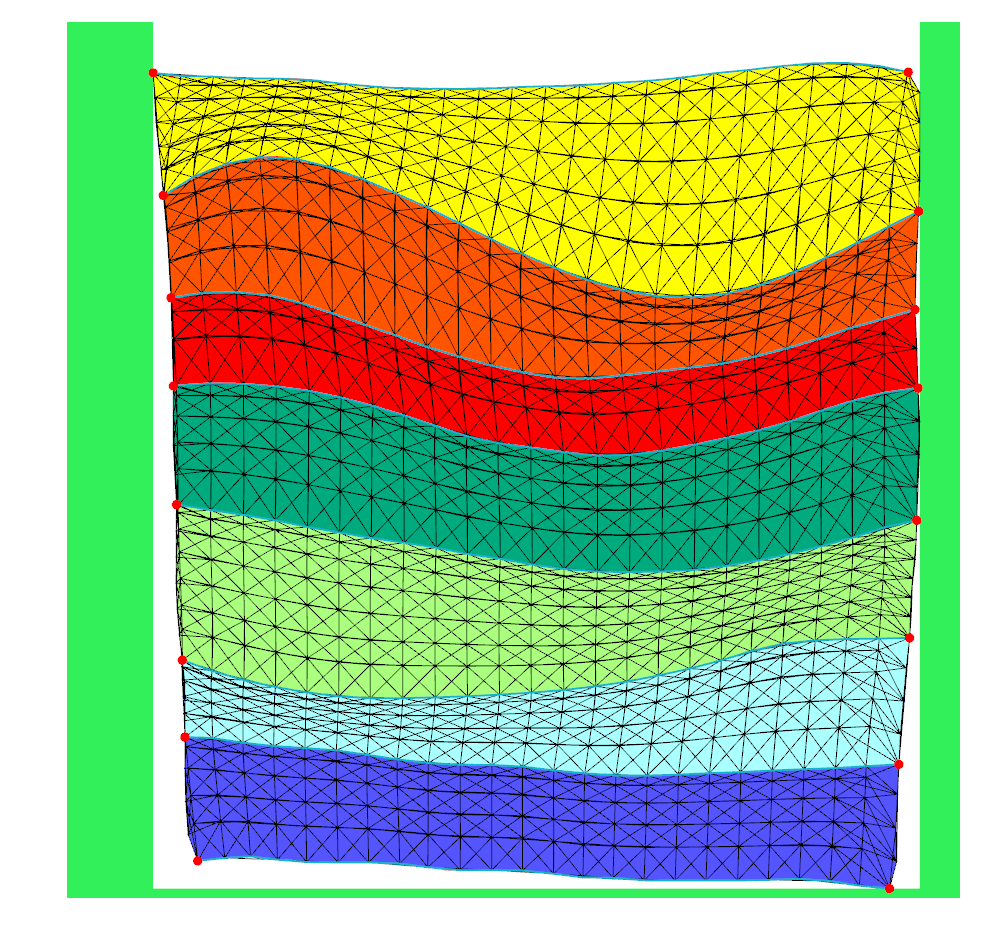
\includegraphics[scale=0.5]{springMapping.png}
	\caption{Mass-Spring Mapping on a layer. In purple: interlayers. In white: sides}
	\end{figure}
	
	
\indent	- The springs we use will also have a torsion resistance in order to accentuate the shape change of the layer.\\\\
In terms of physical equations for a single mass spring system we use the implicit euler scheme and algorithm descibed in \citep{caltech}. We use this scheme instead of an explicit one because it is proven to be more stable with big time step ($dt = 0.02$).\\\\ 
Each particle has the same mass $m$ and possesses at step $n$:\\\\
\indent	- A position  $x_i^n$\\\\
\indent	- A speed $v_i^n$ \\\\\
\indent	- Applied forces $F_i^n$ (containing filtered, corrected and external forces).\\\\
At each time step we will solve the second Newton's law:\\

\begin{align}
	v_i^{n+1} &= v_i^n + F_i^{n+1} \frac{dt}{m}\\
	x_i^{n+1} &= x_i^n + v_i^{n+1} dt 
\end{align}

with:

\begin{equation}
F_i^{n+1} = - \sum\limits_{j|(i,j)\in Edges} k_{ij}(x_i - x_j) + k_{ij}l_{ij}^0\frac{(x_i - x_j)}{||(x_i - x_j)||}
\end{equation}


For each particle we want to integrate the above equations. The problem is that we don't know the forces at step $n + 1$ as we don't know the position of the particles at this step. That is why we use a first order approximation to solve the problem at step $n + 1$:

\begin{equation}
	F^{n+1} = F^n + \frac{\partial F}{\partial x}(x^{n+1} - x^n)
\end{equation}

\noindent Thus we need to compute $H =  \frac{\partial F}{\partial x}$ which is the Jacobian of $F$.\\\\
\noindent By using (1) and (4) we have the following result:
\begin{align*}
	(x^{n+1} - x^n) &= (v^n + (v^{n+1} - v^n))dt \\
	(v^{n+1} - v^n) &= (I - \frac{dt^2}{m}H)^{-1}(F^n + dt H v^n)\frac{dt}{m}
\end{align*}

We now have approximated our equations into a solvable system and we can notice that an additionnal force came from this approximation $dt H v^n$ . It is an implicit viscosity that takes into account the movement of the neighbouring particles.
Consequently we have for each particle $i$ a new force:

\begin{equation}
\tilde{F_i} = k dt \sum\limits_{j|(i,j)\in Edges}(v_j - v_i)
\end{equation}


The last thing to compute is $H$. Like in \citep{caltech} we will approximate $H$ by just integrating the linear part of the elastic force which is equal to:

\begin{equation}
F_{(i,j)} = -k_{ij}(x_i - x_j) + k_{ij}l_{ij}^0\frac{(x_i - x_j)}{||(x_i - x_j)||}
\end{equation}

If $H$ represents only the Jacobian of $F = -k_{ij}(x_i - x_j)$ it has the form:\\
\begin{center}
$
\left\{
\begin{array}{ll}
H_{ij} &= k_{ij} if i \neq j \\
H_{ii} &= -\sum\limits_{j \neq i}k_{ij}
\end{array}
\right.
$
\end{center}

Integrating only the linear part implies that we will have some error at the end of the integration. However we can notice that the non linear part $k_{ij}l_{ij}^0\frac{(x_i - x_j)}{||(x_i - x_j)||}$ has a constant magnitude during the simulation between two steps, so this force just implies a rotation that we will compensiate with another force. Thus we will correct the angular momentum $\delta T$ introduced by this method by adding correcting forces:
\begin{align*}
\delta T &= \sum\limits_{i=1}^n (x_G - x_i)\wedge F_i^{filtered} \\
F_i^{corrected} &= (x_G - x_i)\wedge \delta T dt
\end{align*}

with:
\begin{equation}
F_i^{filtered} = \sum\limits_{i=1}^n F_{ji}W_{ij}
\end{equation}

However in our case the equilibrum length of the springs will change over time creating an error in the angular momentum but we will try compensating this with torsion forces.\\\\

Finally we add torsion forces as external forces (along with gravity) because it is a non linear force and we can't integrate it:

\begin{equation}
F_{ij}^{torsion} = -k_{torsion}\Delta \theta \vec{n}
\end{equation}

with $\Delta \theta$ being the angle between a unit vector depending on the spring type (Vertical, Horizontal, DownShear or UpShear) and the vector $x_i - x_j$. $\vec{n}$ is the normal vector to $x_i - x_j$ pointing toward the unit vector.\\\\
Having this physical structure we will simulate extension and take into account geological features. For the moment we assume that the density and the spring stiffnesses (elastic and torsion) are proportionnal. The friction coefficient will directly be taken into account in the collision computation between faults and particles. As for erosion and sedimentation we will add or remove partcle in the mass-spring system to simulate those events.\\\\
Regarding the extension simulation we will first pull the side where the extension has to occur. This is known before simulating because it is provided by the user. At each time step we will freeze the animation of all the blocks, translate them toward extension apply the physics only to the blocks which are considered to move. The blocks moving undergo either discrete geological event (such as fault) or/and continuous event (erosion or sedimentation). When solving fault apparition we have to stick blocks together. This will be done by attaching corners of the layers when the matching ones are near each other enough. When all the corners are matched we have a new block where we must recompute a new mass spring system.\\\\
Computing a mass spring system can take some time (few seconds for big systems) and can be noticable especially during block fusion but that is not a problem because the goal of the project is to record at each time step the result of our simulation as an inbetween vac which can be played fluently.\\\\

\section{Dealing With Discrete Geological Events}\\

As we mentionned before, geologist are usually able to restore the history of the cross section by using several geometrical and simulation tools.
However then only get one final state of the section whcih represents what was the XS before any techtonic movement. Here we are interested in what 
happened between today XS and the restoration. Indeed most of the time there are several scenarios that lead the initial state to the restoration.
This is what we want in this project. We want to explore the most plausibles scenarios and see the resulting animation of exploration.
To do so we will propose to the user to undo geological events at each time step. We can count already five events to undo : faults, erosion, sedimentation, folding and compaction. Those event will be automatically detected and resbored. In order to solve the issue properlly we'll use two graphs:
	-Story graph
	-Event graph

The Story graph represents the event paths we can run the simulation on. a node represents the list of event we can simulate at time t and an edge represents the event simulated between two nodes. Event graph used in the creation of this graph. It is the graph the user will explorer to see the animation of as many scenarios he wants to see.

Each event has a pre condition and and postcondition and will finish in a state.
Also a event can be have the special property to be dynamic meaining that it will be created during the simulation and not at 
the graphs creation.

The event graph shows time dependencies between geological events. An event is represented by a node and an edge represents a dependency. It is also computed automatically but it can be edited using information provided by the user. Has it contains only dpendencies

Only 4 out of the 5 event have been treated, the compaction will be reserved for later.
Describe the 4 events:

Evaluation functions

Faults: subdivided into modulus event
	Our XS contains what is called fault which corresponds to the breaking of a block into two parts and only two parts. Geologically speaking when a fault begin to open, it splits the block starting by the oldest moduli that is to say from bottom to up. 
	
	We will use this property to decompose our un fault event into several stickModulus events. As we just said the fault split the block into two parts (which are new blocks) and one part is inevitably above the other in terms of y coordinates. Meaning that the corners of each modulus of the upper block is higher than the respecting corners of each modulus of the lower block (see the exemple below). 
	
	As a result the modulus event will correspond to applying forces to the lower block in order to unfold it and make the upper modulus converging to the respecting modulus and then stick together the two moduli when they face each other in terms of y coordinates.
	
	Once all moduli event have ended the fault event can end as well.
	
	-The preconditions are: the fault must concern two blocks and only two blocks. Some faults take root on other ones making them in contact of more than two blocks. 
	
	-The posconditions are: all the modulus events ended mening that all the moduli that should have be stuck together are now merged into one modulus. That implies that the two concerned blocks merged and the mass spring mesh should be regenerated for better uniformity 
	
	How it is done: The fault we want to close is dividing a block into two parts, with one being above the other. We know that the cause of the breaking was folding. Thus we apply to the lower block the exact opposite force that was applied during the folding. For instance if the force applied was a compression pointing toward the left we will apply a force toward the right. Furthermore we have to freeze the movement of the masses of the two concerned blocks that belongs to other faults because we don't want to close those ones yet. Thus if the lower block belongs to another fault the opposite force we apply we create a momentum on the block instead of a translation and will force it being in the same position before the breaking. At the same time the upper block will slowly slide on the lower block causing them to stick together when moduli are at the same high. In addition because of un-detected erosion and small folding events we have to add a additionnal force to the upper block which will make each modulus going toward its corresponding modulus in the lower block. To do so we apply attraction forces $\overrrightarrow{F} = d*\frac{\overrightarrow{(C_{lower} - C_{upper})} }{||\overrightarrow{(C_{lower} - C_{upper})}||}$to the corners of each modulus of the upper block going toward the corresponding corners of the matching modulus. Finally when all the matching moduli have stick together we regenerate the mass-spring system for uniformity sake.

Erode: three types of erosion
	We can identify 4 types of unErode events:
		-unErode youngest moduli :
			here we will search for concavities at the upperside of the youngest moduli and resobe them 
			preconditions : the concerned modulus must be of the youngest material among its block, meaning it is the upper moduli.
			postCondition : the concavities must have been resolved.
			How it is done: Here we look at the upperlayer as being a discretized parametric curve $x(t),y(t)$ and we search for concavities. To do so we will compute the speed vector $x'(t),y'(t)$ and the acceleration vector $x''(t),y''(t)$ and look at the sign of $det(v(t),a(t))$. If it is negative it means that the curve is concave. Thus we search for every concave areas which are intervals $[t_1,t_2]$ where the the curve is concave. Then we have to correct each detected area. To do so we will use hermit curves with the following coefficients $I(t_0), I(t_1)$ which are the points at the beginning and the end of the concavity and $I(t_0) - I(t_0 - 1), I(t_1) - I(t_1 + 1)$  as tangent respectively at point $I(t_0)$ and point $I(t_1)$.Then we deform the current curve making it matching the computed hermit curve. By proceeding this way we will fill the concavities following the trajectory the curve should have if we un-erode it.
			
		- unErode modulus which is in a gap:
			here we will search for up edges which are at the surface but which don't belong to the yongest modulus of the block. Meaning that those edges are the bottom of a hole which is the product of an erosion. We try to resobrbe matter that could have been eroded at those points.
			
			precondition : the modulus must have a edge at the surface without being the youngest modulus of its block
			postcondition: the modulus has been corrected with matter being added.
			
			How it is done: Here we will proceed the exact same way than the previous case except that we won't search for concavities at the upper interlayer but we will try to correct the curve whenever the curve is at the surface, meaning that it joins to corners of younger moduli which are of the same material composition. We will use the corners as starting and ending point of the curve and we will consider the tangent at those point the same way as we computed them previously. Here we don't search for concavities and try to correct the curve in any cases because we can assume than it the concerned modulus was eroded because the erosion divided the modulus jus above it at least in two parts.
		- unErode sides of moduli:
		
			here we are interested at the erosion that happen at the side of moduli and we will also search for concavities in the side of moduli. However we will solve and detect concavities differently than the previous methods because we will take into account the geoloical aspect.
			
			precondition: no preconditions
			postconditions: the side that has been unEroded must not collide with other moduli
			How it is done: Here we will also search for concavities but not at the same place and not the same way than before. First we only look at the left and right side of the modulus here. In fact on these sides there are some concavties that are not due to erosion but just on the way the sediment have deposited and the way the terrain has been fold. Consequently we are only interested at the concavities that only start at the upper corners of the modulus. Then we don't have to compute the derivatives of the curve and we will correct the concavity differently than before. In order to detect the convaties we will consider all the strings between the upper corner (left or right) and the points of the respecting side and see if it intersects the modulus or not. Then we consider the non intersecting string between the upper corner and the side point which is the farthest of the corner in terms of index (if we consider the size having points starting at index $0$ and finishing at index $side_size - 1$). Starting from this side point we will compute the normal at his point and create a new mass following the line beginning at the side point and directed by the normal. The new mass will be created at the point of same high than the upper corner in the line. This point will be the new corner of the modulus and expand it because the side will be moved toward the computed normal line.
		- unErode two moduli of the same material in the same block.
		
		precondition: the moduli must be of the same material and in the same block. In addition they must be facing each other without any modulus between them. 
		postconditions: the gap between the two moduli must have been filled and the mass-spring system msut have been regenerated.
		How it is done: We proceed the same way than the unErode modulus which is in gap case but this time we will not deform an existing curve but we will create a interlayer up between the two concerned moduli using the hermit curve the same way. The starting and ending points will be the corners while the tangent will be the derivatives according to ths neigbouring point.
		

Sediment:

	The preconditions are: if we un sediment one material in all the blocks
	we all the material younger that this one should ahve been unSedimented already. If it is just one molulus we should also check if inside its block there are  no modulus with a material younger than the material of the modulus we want to unSediment.
	
	the postconditions are: the un sedimentation has a duration htat should comes to an end to finish and at the end of the time the concerned moduli should have been erased from the XS. also the massSpring mesh should be reGenerated at the end of the event in order to uniformise the new state of the XS.
	
	How it is done: Here we just reduce gradually the equilibrum length of vertical springs until it reaches zero when we delete the modulus completly. No torsion force will be applied during this animation because we don't want the modulus to undergo deformations.

Fold:
	The preconditions are: there are no precondition for this event. the user is free to play with this event as it allows geologists to test their hypothesis on forces that have been applied to the XS in the past and with a duration.
	
	The posconditions are: the event no longer apply forces on the concerned particles
	
	How it is done: It is quite simple to apply. We add external forces either to a block, a modulus or a specific mass during the requested time. The external forces are taken into account in the main physical loop.
	

\section{Ordonnancing Events}
Branch and Bound
\section{Implementation}
\section{Results}
\section{Limitations}
3D with more drawings
Could have used clothoid
let the user draw erosion line
\section{Conclusion}


III) Geological Structure Representation and Analysis
	How do we represent a Cross Section.
	A Cross-Section contains several parts : 
		-It contains parts of geological layers => floors or moduli
		- A geological layer is a layer composed of the same kind of material.
		In our case we deal with sementary layers. It implies that each material is caracterized by its temporal existance.	
	   	- Faults which can be seen as discontinuities in the XS
		- Blocks which represent the groups of floors delimited by faults.
		- Each Material is caracterised by a Young Modulus which describe its plasticy and elesticity,
		an age period and a friction coefficient.

Drawing analysis. As Mentionned before our input is a colored vpaint drawing which is composed of face, edges and vetices stored in 
a vertex complex graphics strucutre (ref). Passage du sujet.
In the drawing we color faces which represent the different moduli of the XS with the color being its material. moduli of the same color have the same material, therefore they belong to the same layer. We represent interlayers by a white edge while the other contour egades are black. Gaps inside a block are also represented in white and are automatically detected as gaps meaning that erosion impacted this region for sure. line could be added to give hint on the rosion.

Then we have to extract the structure out of this drawing. Meaning that we have to identify the different blocks, moduli, faults and materials from the drawing. To do so we proceed this way: the vpaint output format is an xml file which describe our drawing in terms
of faces, edges and vertices. Each faces has a cycling orientation which is clockwise or counterclockwise but for building and manipulating our structure more easelly we choose that all of our layer will be first read clockwiselly and from the most recent (the higher in general) to the oldest. In fact it is an easy task to wirte the layers in the correct way but we need to find out which layers belong to the same block. To solve this issue we will use the interlayers and then the white edges. Two layers belong to the same block if they share a commun white edge. Thanks to this method we build our blocks. we can notice that the youngest and the oldest layer have just one interlayer that make them part of a block. However we will describe our layer with four part of the contours the upper interlayer, the righedges, the bottom interlayer and the left edges. Consequently for these two specific layer we will compute automatically the lacking interlayer (limitation it is not always good).
	

Hermit curves equations :\\
Given two points $P_0, P_1$ and two tangents $T_0, T_1$ being the tangent we can find at the matching number points, the hermit interpolation which will produce a $C_1$ curve has for equation : 


\begin{equation}
h(t) = (2*t^3 - 3*t^2 + 1)*P_0 + (t^3 - 2*t^2 + t)*T_0 + (t^3 -t^2)*T_1 +(3*t^2 - 2*t^3)*P_0
\end{equation}

It is possible to multiply the tangent by a bias factor which will make the curvature of the curve varying more when this factor becomes big.

Collisions methods: \\

Collisions between blocks. Each layer is delimited by its boundaries which we devide into four parts: upper interlayer, bottom interlayer, right side and left side. Each of these part are composed of segments and the union of all of them is a closed polygon. We deal with block collision by computing particle (circle) segments collision. Moreover for each particle of one block we consider the segement built by the particle position at time $t - dt$ and its position at time $t$ and we check if this segment crosses one of the other blocks segment border. In addition, with this we can also check for collision inside the block it self which is usefull to give reallistic results for un sedimentation for instance. This technique as the advantage of determinig precisely the segment with which the particle collided even if the particle went through the colliding block. However there is still a chance to fail at identifying a collision depending on the order we treat each block animation and collision detection.\\
In order to check intersection between segments we proceed the following way:\\
Given two sgements $[PQ]$ and $[RS]$ we will consider a parametrisation of their equations: 

\begin{align}
	PQ &= P + t*\overrightarrow{PQ} \forall t \in [0,1]\\
	RS &= R + u*\overrightarrow{RS} \forall u \in [0,1]\\
\end{align}

With this parametrisation the two segments intersect if and only if:\\
\begin{equation}
\exists t,u \in [0,1], P + t*\overrightarrow{PQ} = R + u*\overrightarrow{RS}
\end{equation}


We need to extract two equations from this one in order to find $u$ and $t$.
To do so we will use the cross product to keep only one variable in each equation. Thus by applying a cross product with $\overrightarrow{PQ}$ and $\overrightarrow{RS}$ we obtain the following equations:


\begin{align}
	t &= \frac{\overrightarrow{(R - P)} \wedge \overrightarrow{RS}}{\overrightarrow{PQ} \wedge \overrightarrow{RS}}\\
	u &= \frac{\overrightarrow{(P - R)} \wedge \overrightarrow{PQ}}{\overrightarrow{RS} \wedge \overrightarrow{PQ}}
\end{align}

We must note that the simplification was made by noticing that $\overrightarrow{PQ} \wedge \overrightarrow{PQ} = 0$ and $\overrightarrow{RS} \wedge \overrightarrow{RS} = 0$.

Then we can distinguish $4$ cases :
1) $ \overrightarrow{RS} \wedge \overrightarrow{PQ} = 0$ and $\overrightarrow{(P - R)} \wedge \overrightarrow{PQ} = 0$

This means that our segments are parrallel because of the first condition and colinear because of the second. We deduce that our segement are intersecting 
iff :

if ($\overrightarrow{PR}.\overrightarrow{PS} < 0$) or ($\overrightarrow{PR}.\overrightarrow{PS} >= 0$ and $\overrightarrow{PQ}.\overrightarrow{PS} >= 0$ and ($||\overrightarrow{PS}|| < ||\overrightarrow{PQ}||$ or $||\overrightarrow{PR}|| < ||\overrightarrow{PQ}||$))

2)  $ \overrightarrow{RS} \wedge \overrightarrow{PQ} = 0$ and $\overrightarrow{(P - R)} \wedge \overrightarrow{PQ} != 0$
In that case the sgements are parallel but non intersecting.

3)  $ \overrightarrow{RS} \wedge \overrightarrow{PQ} != 0$.
The segment are intersecting iff the computation of $t$ and $u$ gives $t,u \in [0,1]$

4) Otherwise the segements are not parallel and non intersecting


glossary
	
Faults: extensive, inverse (compress), décrochement

Floor, Modulus.

Blocks;

Cross section, 2D slice.

Material.

Young Modulus.

Event: unFolding, unErode, unSediment, un


\bibliography{pfe.bib}

\end{document} 